\documentclass[12pt]{article}
\usepackage[english]{babel}
\usepackage{natbib}
\usepackage{url}
\usepackage[utf8x]{inputenc}
\usepackage{amsmath}
\usepackage{graphicx}
\usepackage{subcaption}
\graphicspath{{images/}}
\usepackage{parskip}
\usepackage{fancyhdr}
\usepackage{vmargin}
\usepackage[shortlabels]{enumitem}


\setmarginsrb{3 cm}{2.5 cm}{3 cm}{2.5 cm}{1 cm}{1.5 cm}{1 cm}{1.5 cm}

\title{Nuclear Medicine Imaging Quality Assurance}					% Title
\author{U.G.C. Jayasankha}								% Author
\date{\today}											% Date
\def \topic{Nuclear Medicine Imaging}

\makeatletter
\let\thetitle\@title
\let\theauthor\@author
\let\thedate\@date
\makeatother

\pagestyle{fancy}
\fancyhf{}
\rhead{\theauthor}
\lhead{\thetitle}
%\chead{170259P}
\cfoot{\thepage}

\begin{document}

%%%%%%%%%%%%%%%%%%%%%%%%%%%%%%%%%%%%%%%%%%%%%%%%%%%%%%%%%%%%%%%%%%%%%%%%%%%%%%%%%%%%%%%%%

\begin{titlepage}
	\centering
    \vspace*{0.5 cm}
    
\includegraphics[scale = 0.8]{University_of_Moratuwa_logo.png}\\[1.0 cm]	% University Logo
    \textsc{\Large Department of Electronics and Telecommunication Engineering}\\[0.8 cm]
    %\textsc{\Large University of Moratuwa}\\[1.0 cm]	% University Name
	\textsc{\large BM 3121}\\[0.5 cm]				% Course Code
	\textsc{\Large Medical Imaging}\\[0.5 cm]				% Course Name
	\rule{\linewidth}{0.2 mm} \\[0.4 cm]
	{ \huge \bfseries \thetitle}\\
	\rule{\linewidth}{0.2 mm} \\[1.5 cm]
	
	\begin{minipage}{0.4\textwidth}
		\begin{flushleft} \large
			\emph{Name:}\\
			\theauthor
			\end{flushleft}
			\end{minipage}~
			\begin{minipage}{0.4\textwidth}
			\begin{flushright} \large
			\emph{Index Number:} \\
			170259P									% Your Student Number
		\end{flushright}
	\end{minipage}\\[2 cm]
	
	{\large \thedate}\\[2 cm]
 
	\vfill
	
\end{titlepage}

%%%%%%%%%%%%%%%%%%%%%%%%%%%%%%%%%%%%%%%%%%%%%%%%%%%%%%%%%%%%%%%%%%%%%%%%%%%%%%%%%%%%%%%%%

\tableofcontents
\pagebreak

%%%%%%%%%%%%%%%%%%%%%%%%%%%%%%%%%%%%%%%%%%%%%%%%%%%%%%%%%%%%%%%%%%%%%%%%%%%%%%%%%%%%%%%%%

\section{Introduction to \topic}
Nuclear Medicine Imaging is a imaging modality which contrasts with other imaging modalities because other modalities focus on providing anatomical details of organs while Nuclear Medicine Imaging focuses on providing details of physiological functions. For that isotopes which emits radiation are injected to the body. 

Nuclear Medicine Imaging is mainly divided into two.
\begin{enumerate}
    \item Single Photon Imaging (SPECT) - Single Gamma rays emitted by radionuclide are detected
    \item Positron Emission Tomography (PET) - Two annihilation photos emitted from positron emitting radionuclide are detected
\end{enumerate}

\begin{figure}[h!]
  \centering
  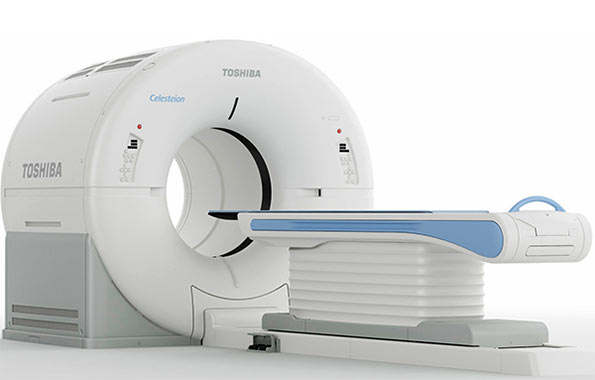
\includegraphics[width=0.6\linewidth]{pet.jpg}
  \caption{\small{PET Scanner}}
  \label{fig:PET Scanner}
\end{figure}

Following figure shows the basic structure of Nuclear Medicine Imaging Scanners. 
\begin{figure}[h!]
  \centering
  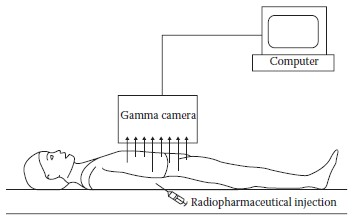
\includegraphics[width=0.5\linewidth]{pet1.jpg}
  \caption{\small{Basic structure of SPECT/PET Scanner}}
  \label{fig:Basic structure of SPECT/PET Scanner}
\end{figure}


\pagebreak
\section{Quality Assurance Aspects of \topic}
In any imaging modality quality assurance is important to ensure the safety of all the people who engages with the scan and to achieve best quality image to diagnose the patient. In Nuclear Medicine Imaging quality assurance should be taken into consideration strictly because of the involvement of radiation and radioactive substances. There is a trade-off between the patients' safety and the quality of the image. Quality assurance methods are required here because of that. There are several topics to be addressed in Nuclear Medicine Imaging quality assurance. 
\begin{itemize}
    \item How to get high quality images 
    \item How to keep the consistency of the image quality
    \item How to ensure the patient safety by using least amount of exposure to radiation
    \item How to minimize the cost
    \item How to increase the efficiency
    \item How to identify errors and repair
\end{itemize}
\begin{figure}[h!]
    \centering
    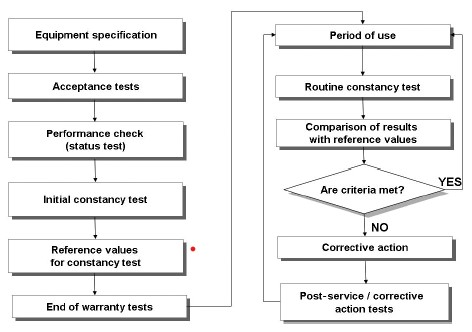
\includegraphics[width=0.65\linewidth]{cycle.jpg}
    \caption{\small{Quality Assurance \& QC cycle}}
    \label{fig:Quality Assurance & QC cycle}
\end{figure}



\section{Phantoms for Nuclear Medicine Imaging QA}
Phantoms are used for quality assurance purposes to measure relevant parameters. In Nuclear Medicine imaging, phantoms are different than others because radioactive substances should be inserted into these. There are several kinds of phantoms used for different quality assurance tests and methods. 


\begin{enumerate}[i.]
    \item Tomographic Uniformity Phantom - Cylindrical Structure with uniform concentration of radioactive substance
    \item Tomographic point source - Spherical structure with point source of radiation at the center
    \item Resolution Phantoms - Point radiation sources are spread all over the structure with uniform attenuation
    \item Total performance phantom - Phantoms with known shapes inside 
    \item A liquid filled flood source
    
\end{enumerate}

\begin{figure}[h!]
    \centering
    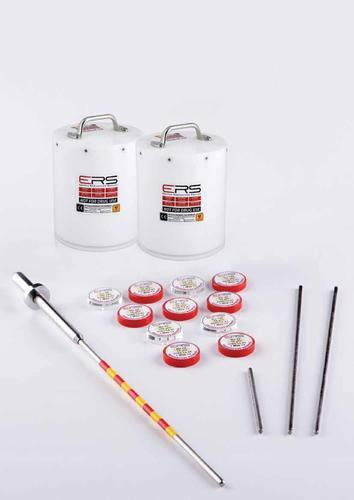
\includegraphics[width=0.45\linewidth]{phantom.jpg}
    \caption{\small{Phantoms and Calibration equipment for PET-CT}}
    \label{fig:Phantoms and Calibration equipment for PET-CT}
\end{figure}
\pagebreak
\begin{figure}[h!]
    \centering
    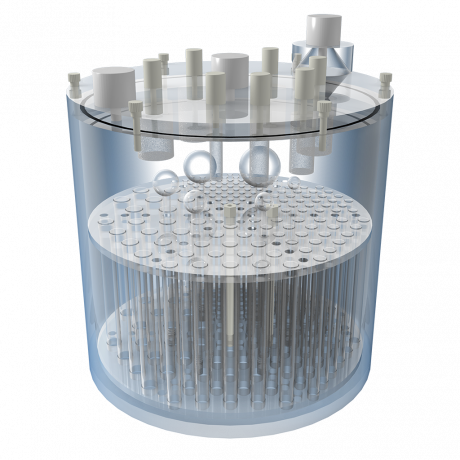
\includegraphics[width=0.55\linewidth]{phantom1.png}
    \caption{\small{Cylindrical phantom}}
    \label{fig:Cylindrical phantom}
\end{figure}



\newpage
\pagebreak
\section{Quality Assurance Methods and Protocols of \topic}
This section describes the main quality assurance methods and protocols used in diagnostic ultrasound. 

\subsection{Quality assurance methods for Hardware}
\subsubsection{Test for Center of Rotation}
Test for center of rotation is to ensure that the physical center of the system coincides with the center computed center of the system using the cameras and collimators. 
\begin{figure}[h!]
    \centering
    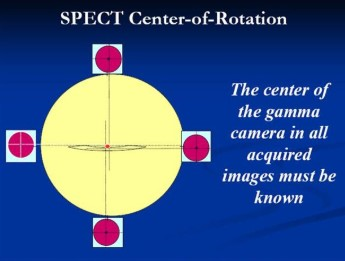
\includegraphics[width=0.45\linewidth]{cor.jpg}
    \caption{\small{Center of rotation - SPECT}}
    \label{fig:Center of rotation - SPECT}
\end{figure}
Procedure of this test is to use all the combinations of cameras and collimators which are used for diagnostic procedures. Corrective measures should be taken if there is a mismatch. 


\subsubsection{Camera Calibration}
Camera calibration is done using uniform distribution phantom. This protocol is to calibrate the radiation intensity measured by scintillation camera according to the actual radiation measured. The phantom used in this protocol has a known radioactivity. Therefore the adjustments are made where the radioactivity converts to the voltage.
\begin{figure}[h!]
    \centering
    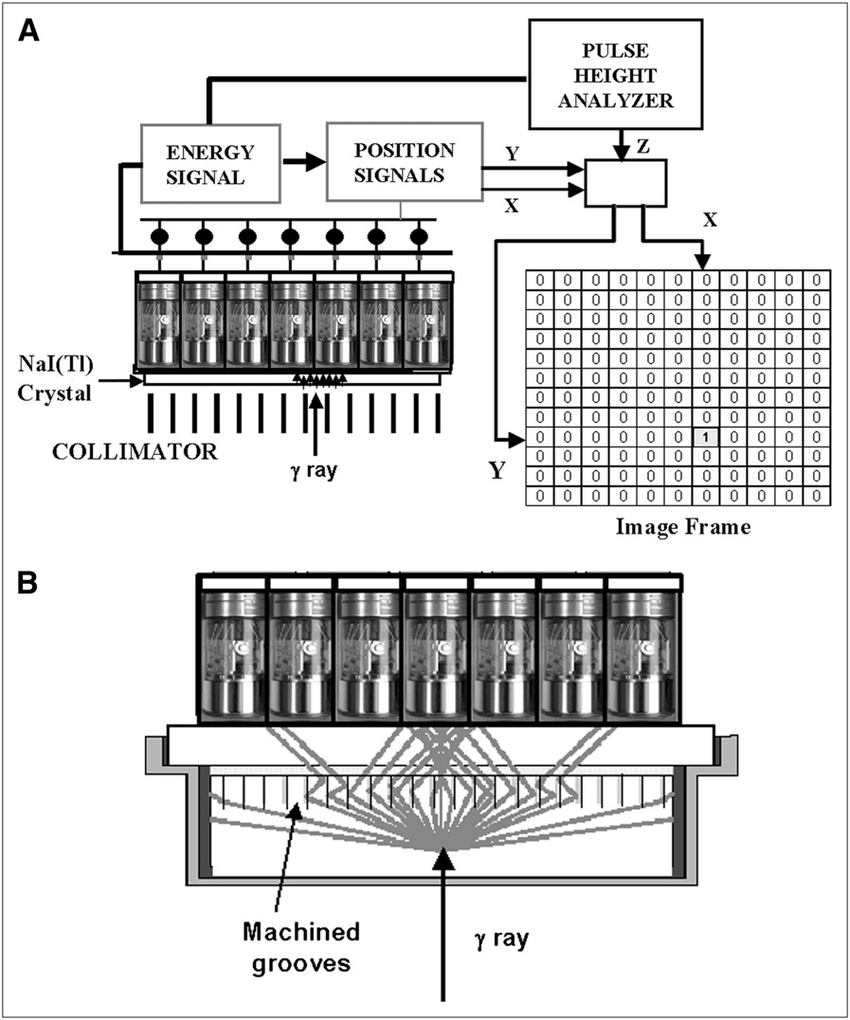
\includegraphics[width=0.45\linewidth]{scc.png}
    \caption{\small{Scintillation Camera}}
    \label{fig:Scintillation Camera}
\end{figure}

\subsection{Quality assurance methods for Imaging system}
% \subsubsection{Spatial Resolution}
\subsubsection{Flood field uniformity}
Flood field uniformity test measures the uniformity of the camera response for a uniform flux of radiation. 
\begin{figure}[h!]
    \centering
    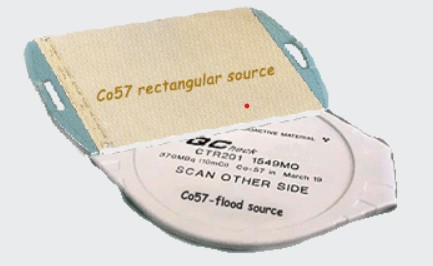
\includegraphics[width=0.45\linewidth]{fs.jpg}
    \caption{\small{Uniform flood source}}
    \label{fig:Uniform flood source}
\end{figure}
A uniform flood phantom is used for this test as shown in above figure. It is uniformly filled Co-57 or Te-99m. A PET scan of this phantom is taken daily and checks for non-uniformity by visual inspection. A quantitative measurement is taken weekly by checking for uniformity by the software. Phantoms should be refilled each time and to maintain uniformity it should be mixed thoroughly.  

\subsubsection{Energy Resolution}
Energy resolution depicts the ability to identify different energy photons. This measurement is made by the intrinsic energy resolution using a point radiation source. For a quantitative measurement multi-channel analyzer is used for the gamma camera. 

Equation for the energy resolution,
\begin{equation*}
    \Delta E (\%) = \frac{FWHME}{E} \times 100
\end{equation*}
FWHME - Width of Photo-peak
E - Photo-peak mean energy

\subsubsection{Shield Leakage Test}
Shield leakage test  is used to measure the gamma camera count rates when exposed to a radioactive source outside the collimator. To check count rates at various points on the shield, a cubic source is used. These count rates are compared with count rate records of the source was placed at 100 mm off from the collimator face.

Leakage count rates calculated by following equation. 
\begin{equation*}
    L (\%) = \frac{Observed\_count\_rate}{Reference\_count\_rate} \times 100\%
\end{equation*}
\begin{figure}[h!]
    \centering
    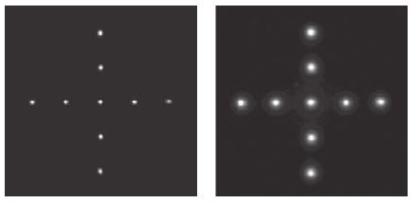
\includegraphics[width=0.45\linewidth]{sh.png}
    \caption{\small{Shield leakage test steps }}
    \label{fig:Shield leakage test steps}
\end{figure}

\subsubsection{Counter rate performance Test}
Maximum count rate capacity and count rate losses of camera can be measured by this test. Standard phantom is used to measure those parameters.


\pagebreak
\subsection{Quality assurance methods for Image quality}
\subsubsection{SNR}
Signal to Noise ratio is one of the most important parameter which shows the quality of the image. Main sources of noise are the deviating system components and moving body parts of the patient. In a high quality image SNR is significantly high with big portion of signal and few noise portion. Signal should be higher than noise component. 
SNR is defined as follows,
\begin{equation*}
    SNR = \frac{Mean\_signal\_intensity}{S.D\_noise}
\end{equation*}

Since windows functions many other functions are used in the system, SNR value based on above equation does not depicts the exaxct amount of noise. Therefore CNR - Contrast to Noise ratio is preferred for that.

\subsubsection{CNR}
Contrast means the ability to distinguish two different things. Here in imaging, contrast is the ability to distinguish two different tissues and identify separately. Contrast to Noise ratio is a measurement of this. A spherical phantom is kept in a volume of fluid of know size containing uniform concentration of radioactive substances. Then the value of pixels in the background of the sphere and the values of pixels inside the sphere can be measured. 

\begin{equation*}
    Contrast = \frac{Value_s_p_h_e_r_e - Value_b_a_c_k_g_r_o_u_n_d}{Value_s_p_h_e_r_e + Value_b_a_c_k_g_r_o_u_n_d}
\end{equation*}

\begin{equation*}
    CNR = \frac{Contrast}{\sigma _b_a_c_k_g_r_o_u_n_d }
\end{equation*}

Basically CNR measures the ability of the imaging system to determine a particular are of different type or activity from the background. 

\subsubsection{Image Uniformity test}
Image Uniformity test is used to ensure that the output of the camera is an uniform image with respect to a uniform object. Uniform sources are used for this test. Generally there is no parameter to determine how uniform the image is. Main reason for the non-uniformity us the attenuation with increasing depth of the phantom. It is measured by the difference of contrast of a symmetrical artefact with respect to a uniform background. 
\begin{figure}[h!]
    \centering
    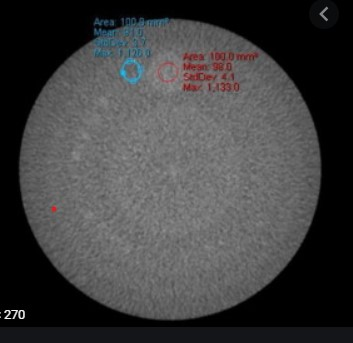
\includegraphics[width=0.45\linewidth]{iu.jpg}
    \caption{\small{Image uniformity test for circular uniform phantom}}
    \label{fig:Image uniformity test for circular uniform phantom}
\end{figure}


\subsubsection{Spatial Resolution}
Spatial resolution is an important parameter which indicates the smallest distance between to objects that can be identified as two objects separately in the image. With time due to exposure for gamma rays, camera losses its ability and spatial resolution is reduced. Thus measuring it is a quality assurance procedure. 

Using transmission or emission phantoms spatial resolution can be qualitatively assessed. 
\begin{figure}[h!]
    \centering
    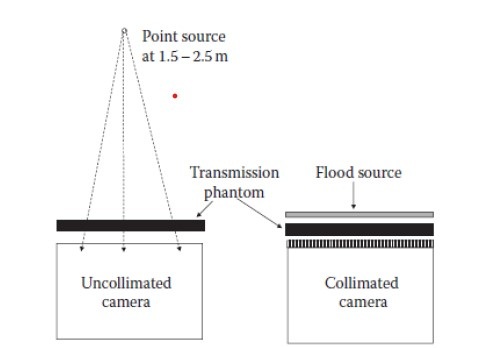
\includegraphics[width=0.65\linewidth]{spa.jpg}
    \caption{\small{+Assessment of spatial resolution}}
    \label{fig:Assessment of spatial resolution}
\end{figure}


\subsubsection{Artefacts}
Artefacts are the objects and ghostly images which can be seen on images but which do not exist physically. This can lead to doctors to wrong interpretations. There are reasons to see artefacts in images. Normally a PET or SPECT scanner comes with a CT scanner built in parallel. In order to use the PET; CT scanner is also used. Therefore artefacts in that system also contribute to the final outcome. 
\begin{figure}[h!]
    \centering
    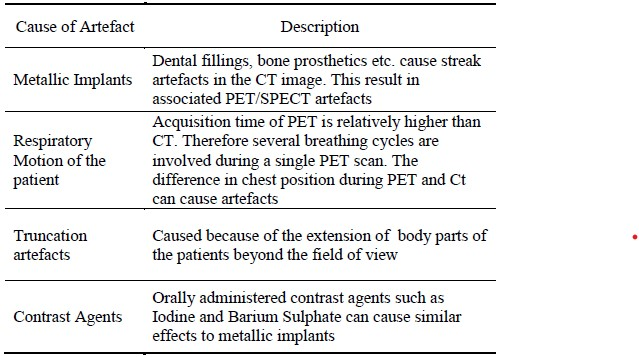
\includegraphics[width=0.85\linewidth]{ar.jpg}
    % \caption{\small{Assessment of spatial resolution}}
    % \label{fig:Assessment of spatial resolution}
\end{figure}


\subsection{Quality assurance methods for display print quality}
This tests are used when the printed images are taken from the same system.


\subsubsection{Display Print quality control}
There can be differences in the image printed on the film and image displayed in the computer display. Quality assurance method is to reduce the deterioration of the image while printing it into a film. 

\begin{figure}[h!]
    \centering
    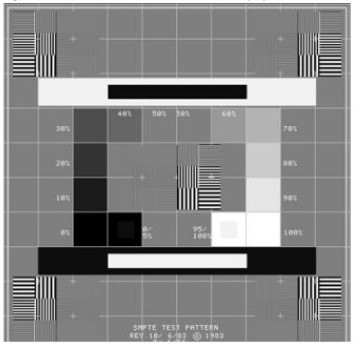
\includegraphics[width=0.65\linewidth]{d.jpg}
    \caption{\small{SMPTE test pattern for Display quality}}
    \label{fig:SMPTE test pattern for Display quality}
\end{figure}

Following figure shows a standard test pattern used for this test. Ii is consisted with several gray scale squares with different intensities. After imaging this, it can be printed onto a film and measure the gray scale values using a densitometer.  

\subsubsection{Display quality control}
Using the same image in the previous topic, this test also can be done. Image is loaded onto the computer display and checked whether the different squares with different gray-scales can be contrasted.If not there is a issue on the Display monitor and needed to be repaired. 

\subsection{Quality assurance methods for Safety measures}
\subsubsection{Background radiation check}
Background radiation check is a daily protocol followed in imaging unit to ensure that the radiation exposure is maintained int the accepted range. This test is important for both the patient and the operator of the scanner. To count the amount of radiation in the imaging room a gamma detector is used. If the radiation level is more than the maximum level of radiation allowed, imaging processes should be stopped and the people inside the room should be evacuated safely. And the room should be decontaminated and should take necessary steps to fix whatever the problem which caused the high amount of radiation in the room.

\pagebreak
\section{Recent advancements in \thetitle}
PET\\SPECT scanners are widely used for cancer detection nowadays. When radioactive medicine are injected to the body, they go through all over the body and stops at places with high metabolism. That means radioactive substances are collected at cancerous cells. Therefore these places are bright spots in the PET/SPECT images. If these bright spots are not spread out all over  body they can be treated and removed. Therefore Nuclear Medicine Imaging is really important for treating cancers. 

Since this procedure requires high contrast to identify small cancerous spots a CT scanner is also attached with the PET scanner. But this combined machine requires new quality assurancce methods and phantoms to be operated. Every parameter discussed earlier should be tested for both systems. There are no specific protocols to check parameters that are results of combination of systems. 
\begin{figure}[h!]
    \centering
    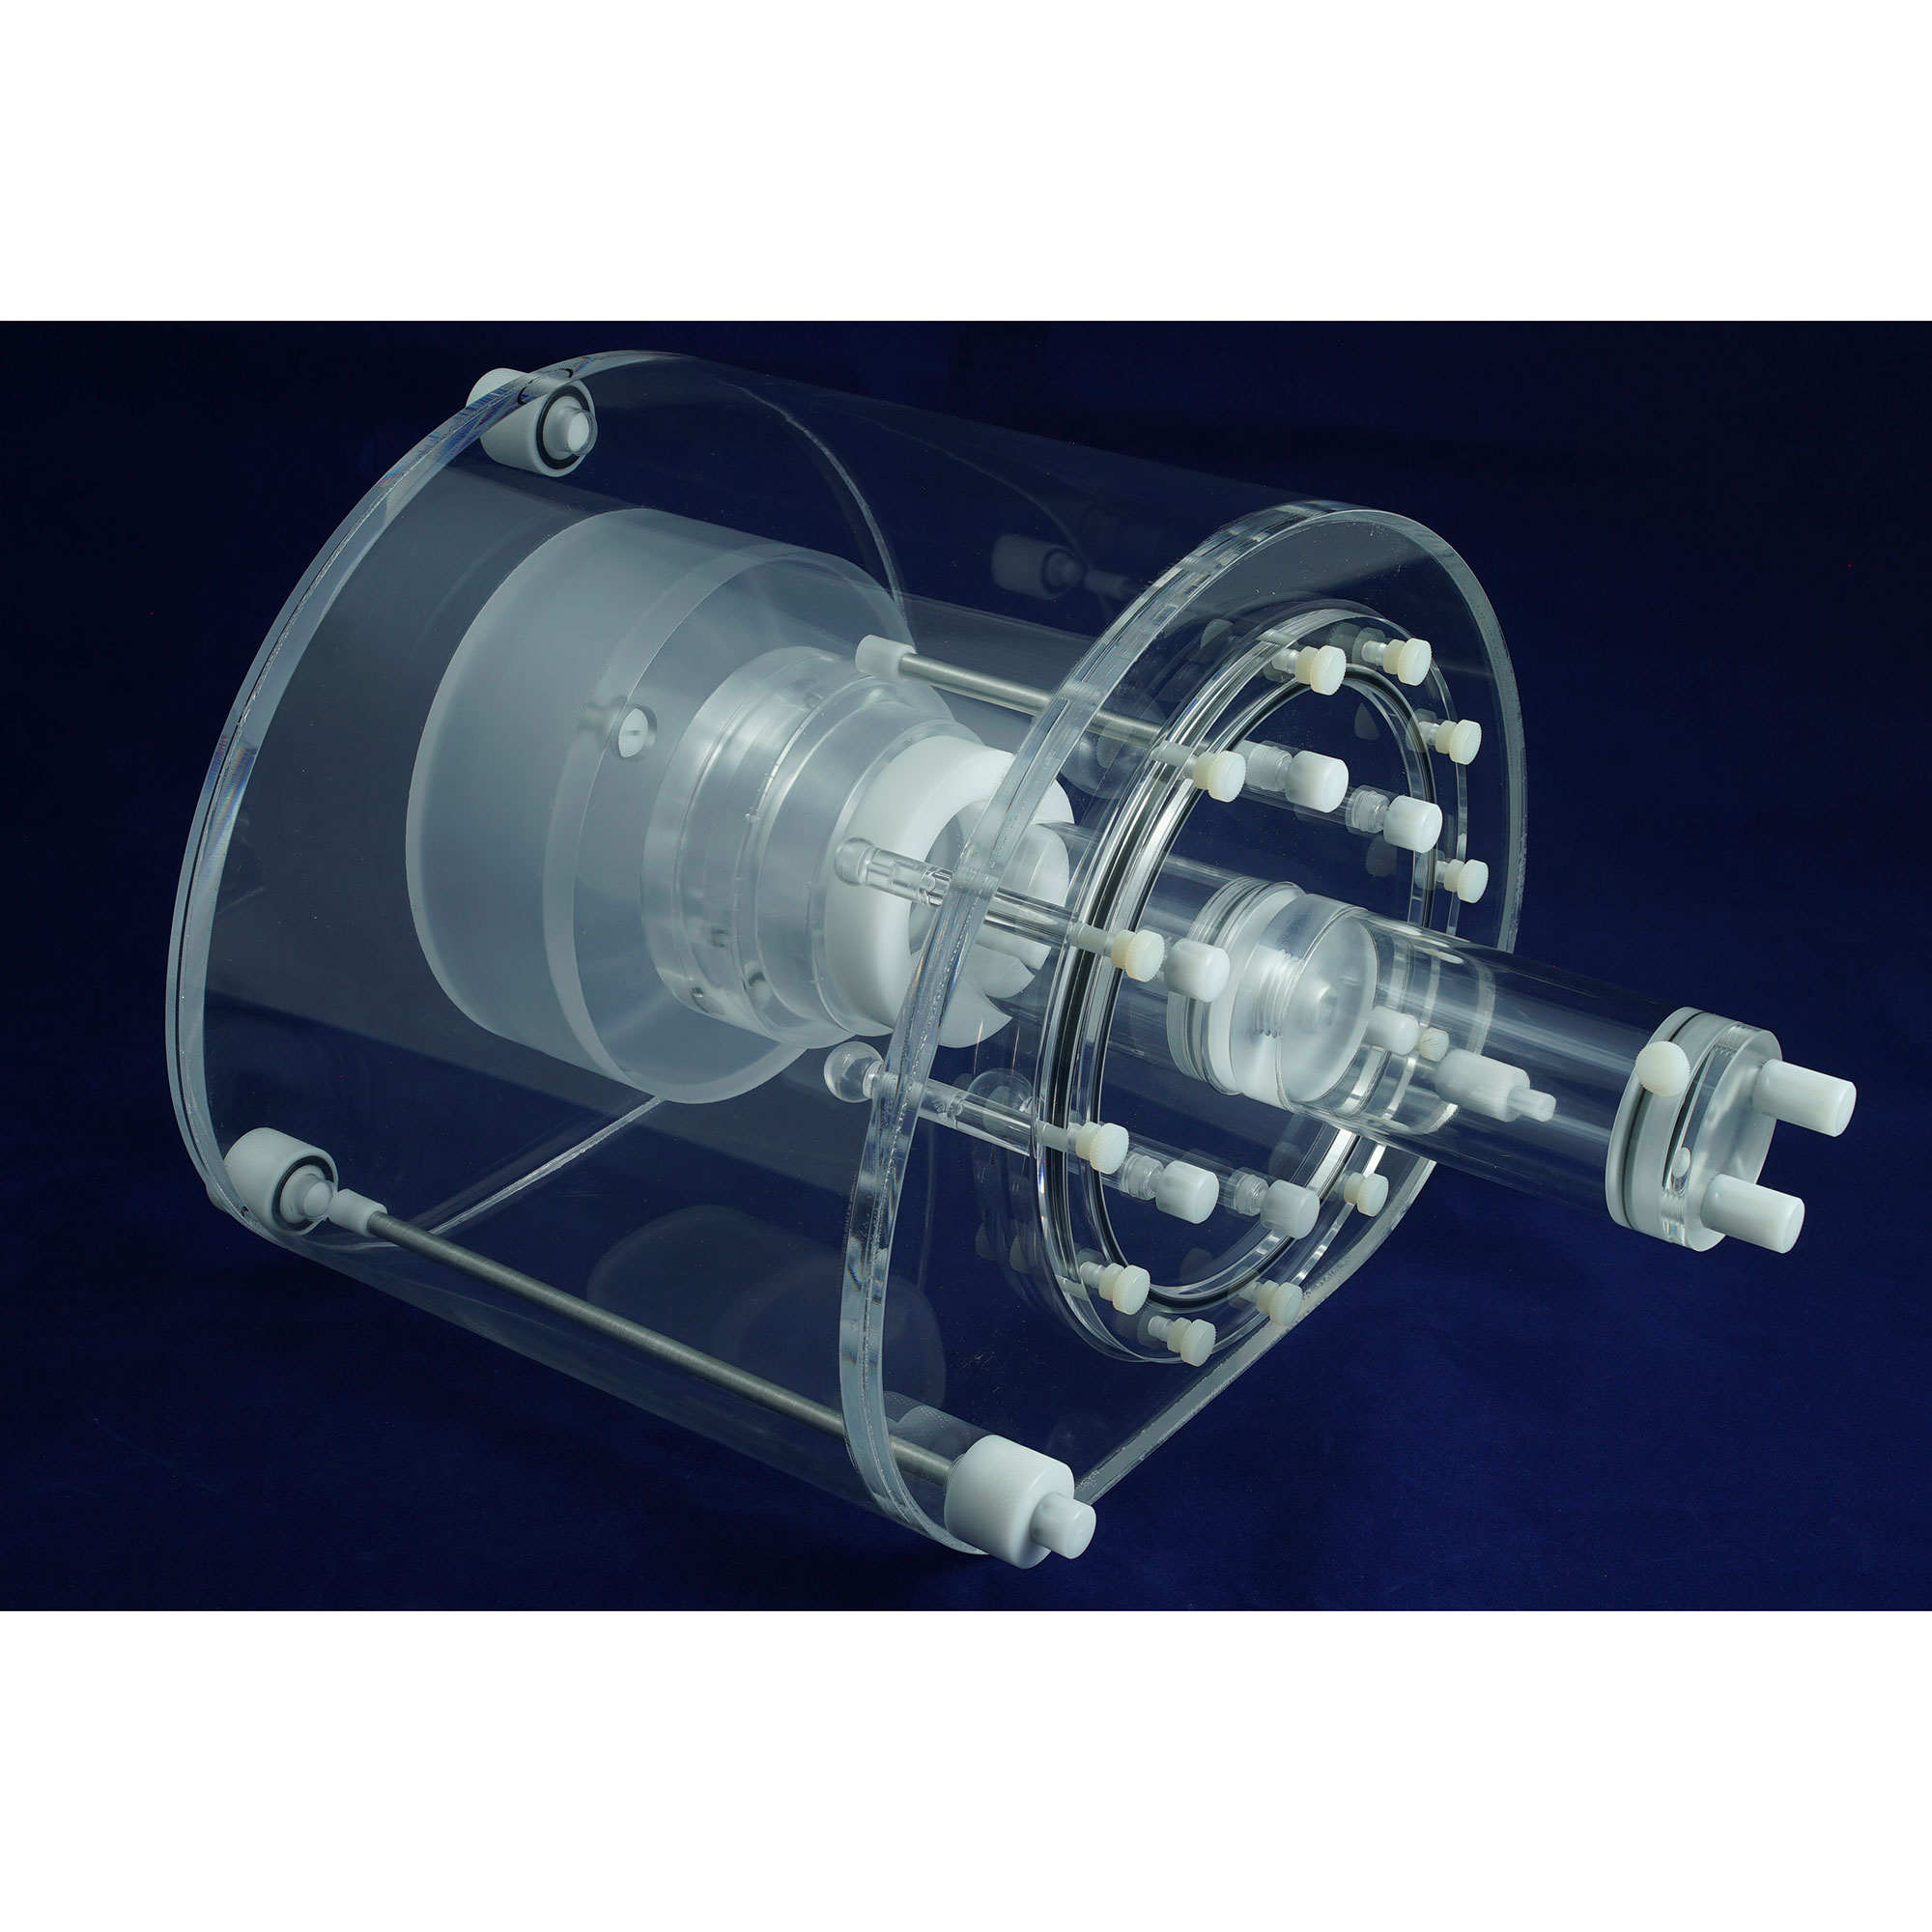
\includegraphics[width=0.65\linewidth]{ct.jpg}
    \caption{\small{PET+CT phantom}}
    \label{fig:PET+CT phantom}
\end{figure}
A new research has developed a phantom to be used in Quality Assurance in CT + PET/SPECT system. It solves most of the problems discussed above. New protocols and Quality assurance methods are published according to this by International Atomic Energy Agency and World Health Organization. 


%\pagebreak
\section{Reference}
\begin{enumerate}

    \item nternational Atomic Energy Agency, QUALITY ASSURANCE FOR PET AND PET/CT SYSTEMS, Vienna: IAEA, 2009.
    \item P. Keim, "An Overview of PET Quality Assurance Procedures: Part 1," Journal of Nuclear Medicine Technology, vol. 22, no. 1, pp. 27-34, 1994. 
    \item A. R. Webb, Introduction to biomedical imaging. Hoboken, N. J.: John Wiley \& Sons, 2006.
    \item Internation Atomic Energy Agency, Quality Assurance for SPECT Systems, Vienna: IAEA, 2009.
    \item “Home,” RSS. [Online]. Available: http://www.aapm.org/. [Accessed: 18-May-2020].
    \item Biodex, "PET Phantoms," Biodex, [Online]. Available: http://www.biodex.com/nuclear-medicine/products/pet-positron-emission-tomography/pet-phantoms. [Accessed 23 05 2020].
    
    
\end{enumerate}
\pagebreak
\textbf{\Large{Appendix}}
\begin{appendix}
  \listoffigures
  %\listoftables
\end{appendix}

\end{document}


